\subsection{Opgave 30}

På figuren ses grafen for et andengradspolynomium på formen $f(x) = a\cdot x^2 +b\cdot x + c$.

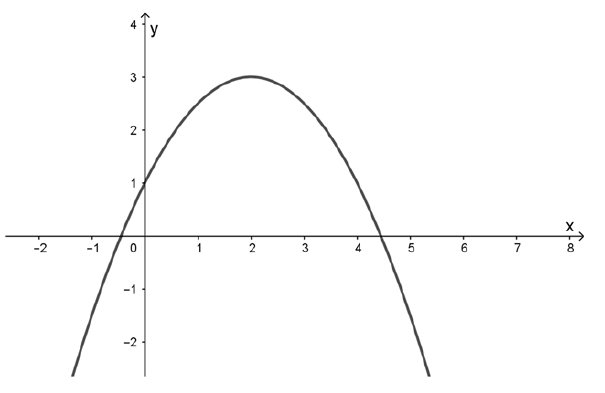
\includegraphics[width=8cm]{Opgave_21-30/Opgave_30/30.png}

Bestem fortegnet for a, og bestem fortegnet for c.

\ans

For et andengradspolynomium fortæller fortegnet af a om vores polynomie vender opad eller nedad.
Da andengradspolynomiet på figuren vender nedad er fortegnet for a dermed negativt.

For et andengradspolynomium er c værdien der hvor polynomiet skærer y aksen.
Da andengradspolynomiet på figuren skærer y aksen i $y = 1$ er fortegnet for c dermed positivt.


